
\chapter{System Testing during Stress Test}

\section{Overview}

Two patients wore the system while performing a stress test on the treadmill following the modified Bruce protocol. Information about heart rate and motion was recorded by the proposed system and hospital equipment.

The objective of this experiment was to compare the reliability of various sources of HR and METs values.

During the experiment, patient wore both, the proposed system and hospital's equipment, which caused some problems with electrode placement and, in some periods, lead to the loss of ECG data due to a bad contact between the chest band and the skin.

\FloatBarrier
\section{Results}

Data from hospital equipment is available from two sources, in files with a sampling rate of 1 sample/min or in the form of plots saved as images. From this images, data was traced with higher sampling rate, although this manual tracing, inevitably, introduced some error to the values recovered.

\begin{figure}[!h]
	\centering
	\makebox[\linewidth][c]{%
		\begin{subfigure}[t]{0.55\textwidth}
			\centering
			\captionsetup{width=.75\linewidth}
			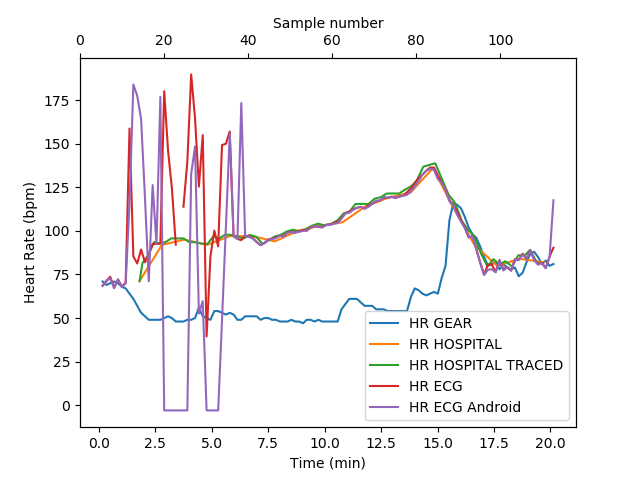
\includegraphics[width=\textwidth]{hr-android-4-4.png}
			\caption{Subject 1}
		\end{subfigure}%
		\begin{subfigure}[t]{0.55\textwidth}
			\centering
			\captionsetup{width=.75\linewidth}
			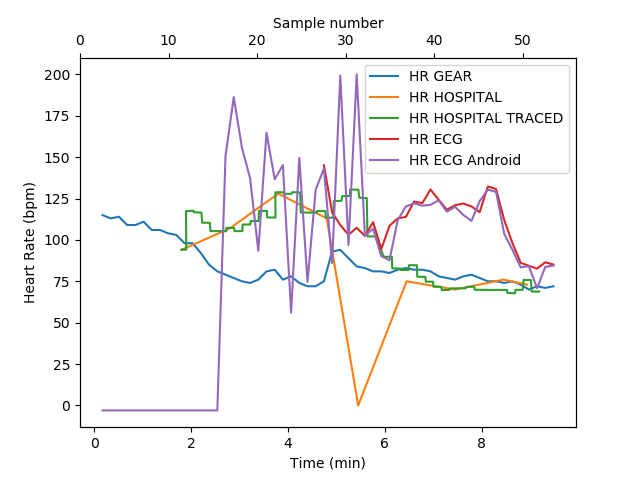
\includegraphics[width=\textwidth]{hr-android-5-5.png}
			\caption{Subject 2}
		\end{subfigure}%
	}\\

	\caption{Heart Rate calculated from various sources: (blue) Gear's algorithm; (orange) Values returned from hospital equipment; (green) Values traced from plot printed by hospital equipment; (red) State of the art ECG segmenter; (purple) Simplified segmenter implemented in phone}

	\makebox[\linewidth][c]{%
		\begin{subfigure}[t]{0.55\textwidth}
			\centering
			\captionsetup{width=.75\linewidth}
			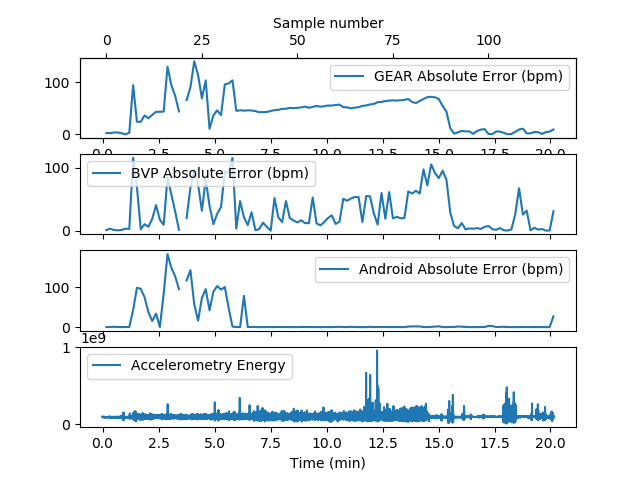
\includegraphics[width=\textwidth]{erro-android-4-4.png}
			\caption{Subject 1}
			\label{fig:hosp-hr-4}
		\end{subfigure}%
		\begin{subfigure}[t]{0.55\textwidth}
			\centering
			\captionsetup{width=.75\linewidth}
			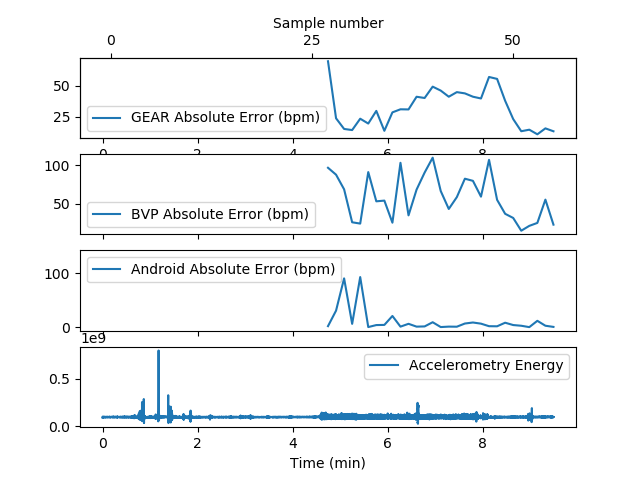
\includegraphics[width=\textwidth]{erro-android-5-5.png}
			\caption{Subject 2}
			\label{fig:hosp-hr-5}
		\end{subfigure}%
	}\\

	\caption{Error from the various methods using state of the art segmenter as ground truth (hospital data was not compared due to different sampling rate)}

	\makebox[\linewidth][c]{%
		\begin{subfigure}[t]{0.55\textwidth}
			\centering
			\captionsetup{width=.75\linewidth}
			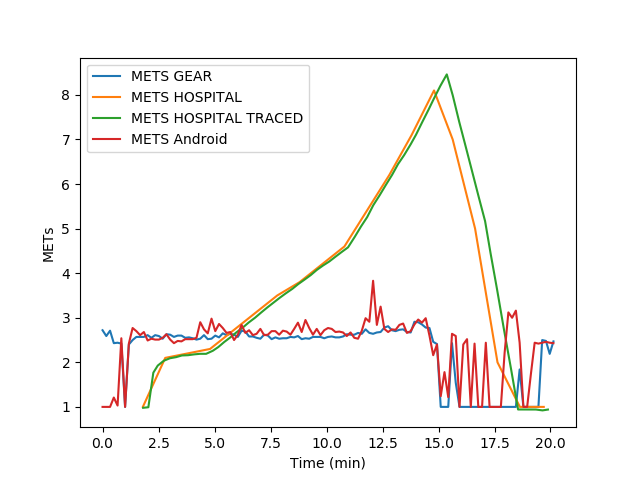
\includegraphics[width=\textwidth]{mets-android-4-4.png}
			\caption{Subject 1}
		\end{subfigure}%
		\begin{subfigure}[t]{0.55\textwidth}
			\centering
			\captionsetup{width=.75\linewidth}
			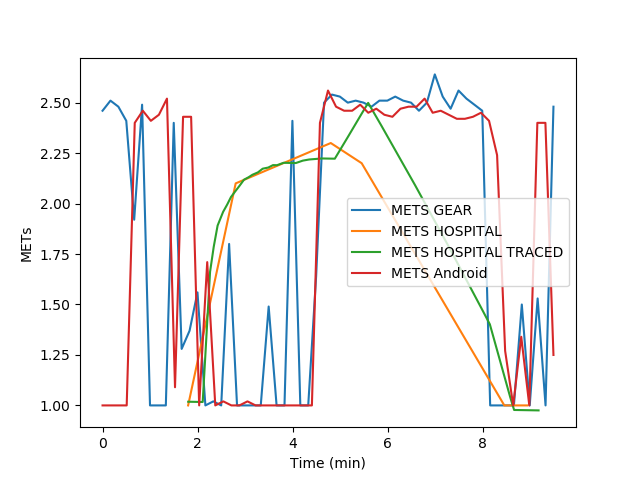
\includegraphics[width=\textwidth]{mets-android-5-5.png}
			\caption{Subject 2}
		\end{subfigure}	%
	}\\

	\caption{METs determined from different sources:  (blue) Gear's accelerometer; (orange) Values returned from hospital equipment; (green) Values traced from plot printed by hospital equipment; (red) Phone accelerometer}

	\label{fig:hosp}
\end{figure}

%RAW
\begin{figure}[!h]
	\centering
	\makebox[\linewidth][c]{%
		\begin{subfigure}[t]{0.55\textwidth}
			\centering
			\captionsetup{width=.75\linewidth}
			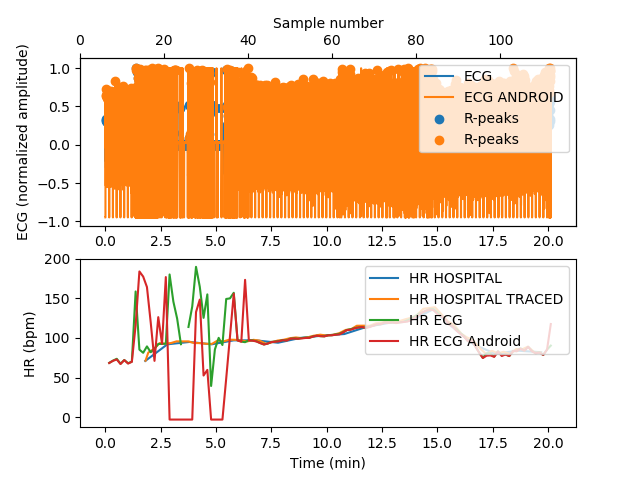
\includegraphics[width=\textwidth]{ecg-4-4.png}
			\caption{Subject 1}
			\label{fig:hosp-raw-4}
		\end{subfigure}%
		\begin{subfigure}[t]{0.55\textwidth}
			\centering
			\captionsetup{width=.75\linewidth}
			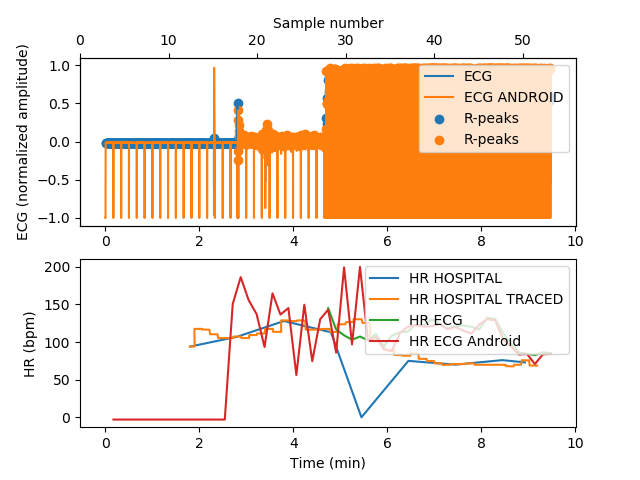
\includegraphics[width=\textwidth]{ecg-5-5.png}
			\caption{Subject 2}
			\label{fig:hosp-raw-5}
		\end{subfigure}%
	}\\
	
	\caption{Raw ECG acquired by the chest band when processed by android segmenter (blue) and by a state of the art algorithm (orange)}
	
	\makebox[\linewidth][c]{%
		\begin{subfigure}[t]{0.55\textwidth}
			\centering
			\captionsetup{width=.75\linewidth}
			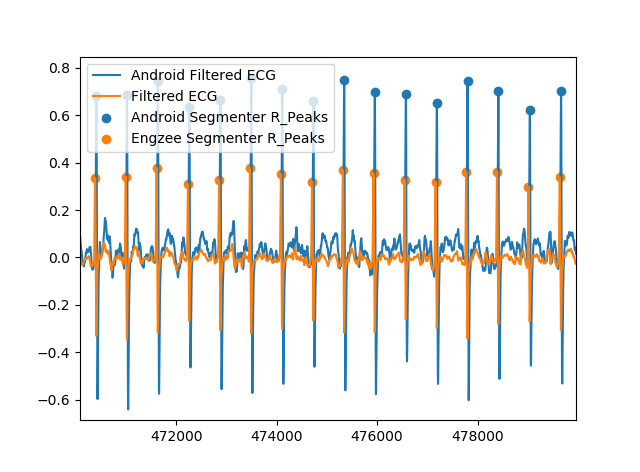
\includegraphics[width=\textwidth]{ecg-4-4-good.png}
			\caption{Subject 1 - ECG segment used to calculate sample nr 50 of HR (\cref{fig:hosp-hr-4})}
		\end{subfigure}%
		\begin{subfigure}[t]{0.55\textwidth}
			\centering
			\captionsetup{width=.75\linewidth}
			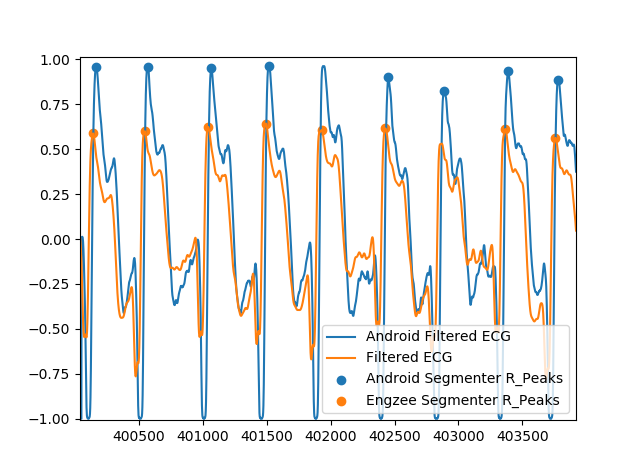
\includegraphics[width=\textwidth]{ecg-5-5-good.png}
			\caption{Subject 2 - ECG segment used to calculate sample nr 43 of HR (\cref{fig:hosp-hr-5})}
		\end{subfigure}%
	}\\

	\caption{Example of ECG segments used to calculate HR with small error}
	
	\makebox[\linewidth][c]{%
		\begin{subfigure}[t]{0.55\textwidth}
			\centering
			\captionsetup{width=.75\linewidth}
			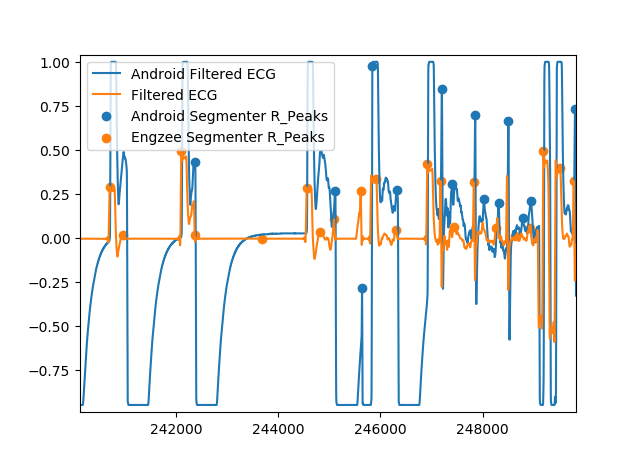
\includegraphics[width=\textwidth]{ecg-4-4-bad.png}
			\caption{Subject 1 - ECG segment used to calculate sample nr 25 of HR (\cref{fig:hosp-hr-4})}
		\end{subfigure}%
		\begin{subfigure}[t]{0.55\textwidth}
			\centering
			\captionsetup{width=.75\linewidth}
			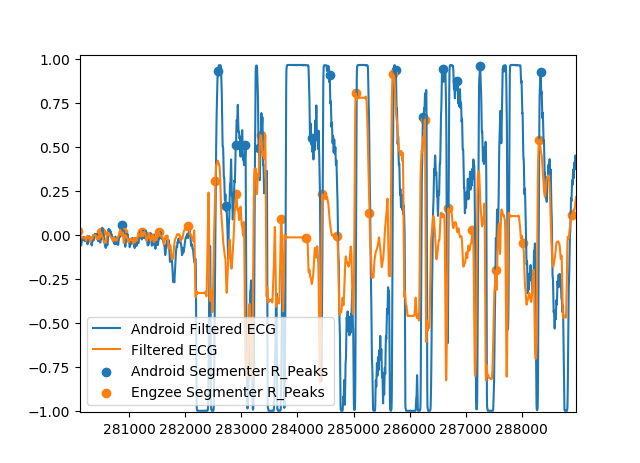
\includegraphics[width=\textwidth]{ecg-5-5-bad.png}	
			\caption{Subject 2 - ECG segment used to calculate sample nr 16 of HR (\cref{fig:hosp-hr-5})}
			\label{fig:hosp-raw-5-bom}
		\end{subfigure}	%
	}\\

	\caption{Example of ECG segments used to calculate HR with big error}
		
	\label{fig:hosp-raw}
\end{figure}


\FloatBarrier
\section{Conclusions}

As can be seen in \cref{fig:hosp-raw-5-bom} even when android and the state of the art algorithm detect the same R-peaks, which should indicate both are correct, the HR value obtained still is very different from the one returned by the hospital's equipment. This could indicate that ECG electrode placement was interfering with the ECG acquisition by the chest band. This hypothesis is supported by the fact that during approximately half of the experiment with subject 2, no ECG was acquired as can be seen in 	\cref{fig:hosp-raw-5}.

For Subject 1, although the electrode placement was still a problem, the ECG signal had good quality the majority of the time, allowing the algorithms to produce good results.

Regarding METs calculation, the results had significant error. This can be caused by several factors. One could be having subjects walking in a treadmill, which presents a fairly different accelerometer compared to really walking. 
%Another reason could be the calculation of METs by the hospital equipment that is(?) an estimation and not a measured value, this could introduce error as this estimation could be biased and not correspond to reality.


